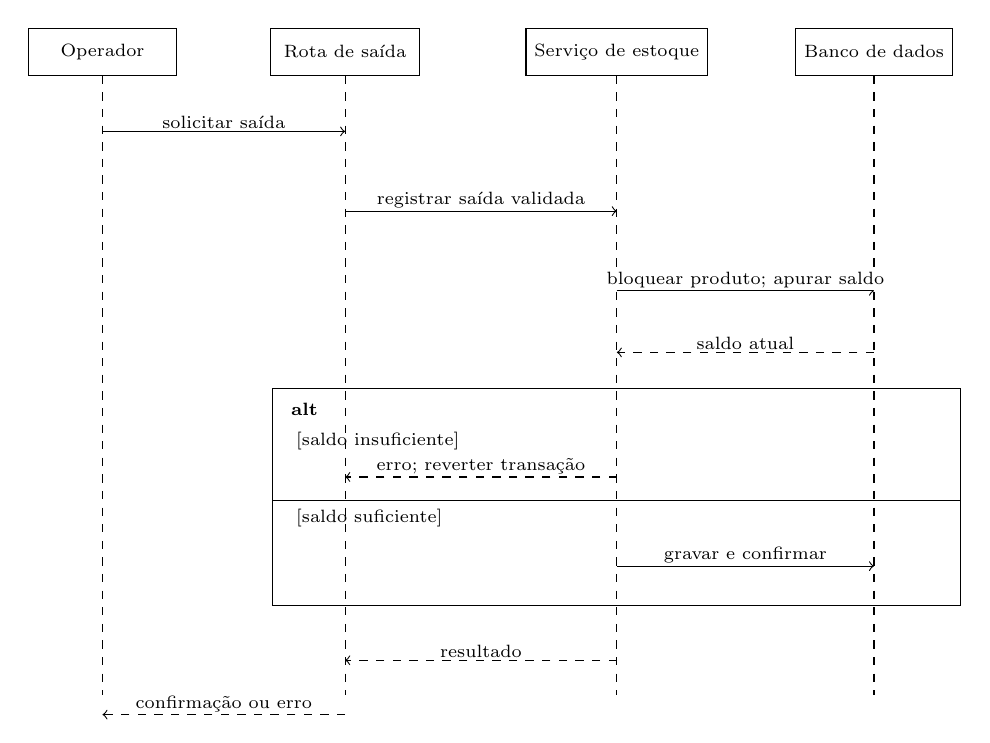
\begin{tikzpicture}[x=1cm,y=1cm,scale=0.92,transform shape,
  participante/.style={draw,rectangle,align=center,minimum width=2.05cm,minimum height=.65cm,font=\scriptsize},
  mensagem/.style={->,thin}, retorno/.style={->,thin,dashed},
  rotulo/.style={font=\scriptsize,fill=white,inner sep=1pt}]
  \node[participante] (u) at (0,9.2) {Operador};
  \node[participante] (r) at (3.35,9.2) {Rota de saída};
  \node[participante] (s) at (7.1,9.2) {Serviço de estoque};
  \node[participante] (b) at (10.65,9.2) {Banco de dados};
  \foreach \n in {u,r,s,b} \draw[dashed] (\n.south)--++(0,-8.55);
  \draw[mensagem] (0,8.1)--node[rotulo,above]{solicitar saída} (3.35,8.1);
  \draw[mensagem] (3.35,7.0)--node[rotulo,above]{registrar saída validada} (7.1,7.0);
  \draw[mensagem] (7.1,5.9)--node[rotulo,above]{bloquear produto; apurar saldo} (10.65,5.9);
  \draw[retorno] (10.65,5.05)--node[rotulo,above]{saldo atual} (7.1,5.05);
  \draw (2.35,4.55) rectangle (11.85,1.55);
  \node[anchor=north west,font=\scriptsize\bfseries] at (2.48,4.48) {alt};
  \node[anchor=west,font=\scriptsize] at (2.55,3.83) {[saldo insuficiente]};
  \draw[retorno] (7.1,3.33)--node[rotulo,above]{erro; reverter transação} (3.35,3.33);
  \draw (2.35,3.0)--(11.85,3.0);
  \node[anchor=west,font=\scriptsize] at (2.55,2.76) {[saldo suficiente]};
  \draw[mensagem] (7.1,2.1)--node[rotulo,above]{gravar e confirmar} (10.65,2.1);
  \draw[retorno] (7.1,.8)--node[rotulo,above]{resultado} (3.35,.8);
  \draw[retorno] (3.35,.05)--node[rotulo,above]{confirmação ou erro} (0,.05);
\end{tikzpicture}
